\documentclass{vgtc}                          % final (conference style)
%\documentclass[review]{vgtc}                 % review
%\documentclass[widereview]{vgtc}             % wide-spaced review
%\documentclass[preprint]{vgtc}               % preprint
%\documentclass[electronic]{vgtc}             % electronic version

%% Uncomment one of the lines above depending on where your paper is
%% in the conference process. ``review'' and ``widereview'' are for review
%% submission, ``preprint'' is for pre-publication, and the final version
%% doesn't use a specific qualifier. Further, ``electronic'' includes
%% hyperreferences for more convenient online viewing.

%% Please use one of the ``review'' options in combination with the
%% assigned online id (see below) ONLY if your paper uses a double blind
%% review process. Some conferences, like IEEE Vis and InfoVis, have NOT
%% in the past.

%% Figures should be in CMYK or Grey scale format, otherwise, colour 
%% shifting may occur during the printing process.

%% These few lines make a distinction between latex and pdflatex calls and they
%% bring in essential packages for graphics and font handling.
%% Note that due to the \DeclareGraphicsExtensions{} call it is no longer necessary
%% to provide the the path and extension of a graphics file:
%% \includegraphics{diamondrule} is completely sufficient.
%%
\ifpdf%                                % if we use pdflatex
  \pdfoutput=1\relax                   % create PDFs from pdfLaTeX
  \pdfcompresslevel=9                  % PDF Compression
  \pdfoptionpdfminorversion=7          % create PDF 1.7
  \ExecuteOptions{pdftex}
  \usepackage{graphicx}                % allow us to embed graphics files
  \DeclareGraphicsExtensions{.pdf,.png,.jpg,.jpeg} % for pdflatex we expect .pdf, .png, or .jpg files
\else%                                 % else we use pure latex
  \ExecuteOptions{dvips}
  \usepackage{graphicx}                % allow us to embed graphics files
  \DeclareGraphicsExtensions{.eps}     % for pure latex we expect eps files
\fi%

%% it is recomended to use ``\autoref{sec:bla}'' instead of ``Fig.~\ref{sec:bla}''
\graphicspath{{figures/}{pictures/}{images/}{figures/study/}{./}} % where to search for the images

\usepackage{microtype}                 % use micro-typography (slightly more compact, better to read)
\PassOptionsToPackage{warn}{textcomp}  % to address font issues with \textrightarrow
\usepackage{textcomp}                  % use better special symbols
\usepackage{mathptmx}                  % use matching math font
\usepackage{times}                     % we use Times as the main font
\renewcommand*\ttdefault{txtt}         % a nicer typewriter font
\usepackage{cite}                      % needed to automatically sort the references
\usepackage{tabu}                      % only used for the table example
\usepackage{booktabs}                  % only used for the table example
\usepackage{color}
%% We encourage the use of mathptmx for consistent usage of times font
%% throughout the proceedings. However, if you encounter conflicts
%% with other math-related packages, you may want to disable it.


%% If you are submitting a paper to a conference for review with a double
%% blind reviewing process, please replace the value ``0'' below with your
%% OnlineID. Otherwise, you may safely leave it at ``0''.
\onlineid{0}

%% declare the category of your paper, only shown in review mode
\vgtccategory{Research}

%% allow for this line if you want the electronic option to work properly
\vgtcinsertpkg

%% In preprint mode you may define your own headline.
%\preprinttext{To appear in an IEEE VGTC sponsored conference.}

%% Paper title.

\title{Visual Analysis of Ligand Trajectories in Molecular Dynamics}

%% This is how authors are specified in the conference style

%% Author and Affiliation (single author).
%%\author{Roy G. Biv\thanks{e-mail: roy.g.biv@aol.com}}
%%\affiliation{\scriptsize Allied Widgets Research}

%% Author and Affiliation (multiple authors with single affiliations).
%%\author{Roy G. Biv\thanks{e-mail: roy.g.biv@aol.com} %
%%\and Ed Grimley\thanks{e-mail:ed.grimley@aol.com} %
%%\and Martha Stewart\thanks{e-mail:martha.stewart@marthastewart.com}}
%%\affiliation{\scriptsize Martha Stewart Enterprises \\ Microsoft Research}

%% Author and Affiliation (multiple authors with multiple affiliations)
\author{Adam Jur\v{c}\'{i}k\thanks{e-mail: xjurc@fi.muni.cz}\\ %
        \scriptsize Masaryk University %
\and Katar\'{i}na Furmanov\'{a}\\ %
     \scriptsize Masaryk University %
\and Jan By\v{s}ka\\ %
     \parbox{1.4in}{\scriptsize \centering University of Bergen \\ Masaryk University} %
\and Vojt\v{e}ch Von\'{a}sek\\ %
     \scriptsize Czech Technical University %
\vspace{\baselineskip} %
\and Ond\v{r}ej V\'{a}vra\\ %
     \scriptsize Masaryk University %
\and Pavol Ulbrich\\ %
     \scriptsize Masaryk University
\and Helwig Hauser\\ %
     \scriptsize University of Bergen %
\and Barbora Kozl\'{i}kov\'{a}\\ %
     \scriptsize Masaryk University}

%% A teaser figure can be included as follows, but is not recommended since
%% the space is now taken up by a full width abstract.
%\teaser{
%  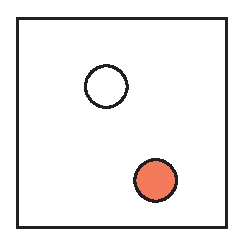
\includegraphics[width=1.5in]{sample.eps}
%  \caption{Lookit! Lookit!}
%}

%% Abstract section.
\abstract{
Exploration of protein reactivity with other molecules plays a crucial role in many biochemical research disciplines, including protein engineering and drug design.
In many cases, a small molecule (ligand) reacts with the protein in its deeply buried active site. 
As the ligand has to be transported to this site from the protein outer environment, it is crucial to study trajectories, which the ligand can follow.
There are several in-silico methods, enabling to calculate potential trajectories in a protein model.
When these methods are applied in connection with molecular dynamics simulation, usually large ensembles of trajectories are produced.
These trajectories have to be further explored by the biochemists who are trying to assess their relevance and gain insight into the protein function.
During this process, many parameters of the trajectories have to be taken into account.
This makes the exploration very demanding as the biochemists have to analyze the multidimensional data about trajectories.
Without proper visual support, this process is very complicated and time demanding.
In this paper, we introduce a novel tool for visual analysis of ligand trajectories and their various properties.
The tool has been designed in tight collaboration with the domain experts in order to address their needs as much as possible.
It is composed of several 2D and 3D linked views, enabling interactive exploration and filtering of trajectories.
%The tool consists of a set of 2D views and the 3D view.
It utilizes the concept of small multiples for communicating the properties of the trajectories.
Through a variety of interaction techniques, the system enables users to create and store selections that can be compared and evaluated later.
In both 2D and 3D views, users can either observer the individual trajectories or choose to aggregate the information into a functional boxplot or a density visualization.
%It utilizes the concept of a scatterplot matrix for communicating different properties of the trajectories.
The usefulness of the tool is demonstrated in two case studies, conducted by the collaborating protein engineers.
} % end of abstract

%% ACM Computing Classification System (CCS). 
%% See <http://www.acm.org/about/class> for details.
%% We recommend the 2012 system <http://www.acm.org/about/class/class/2012>
%% For the 2012 system use the ``\CCScatTwelve'' which command takes four arguments.
%% The 1998 system <http://www.acm.org/about/class/class/2012> is still possible
%% For the 1998 system use the ``\CCScat'' which command takes four arguments.
%% In both cases the last two arguments (1998) or last three (2012) can be empty.

\CCScatlist{
  \CCScatTwelve{Human-centered computing}{Visu\-al\-iza\-tion}{Visu\-al\-iza\-tion techniques}{Treemaps};
  \CCScatTwelve{Human-centered computing}{Visu\-al\-iza\-tion}{Visualization design and evaluation methods}{}
}

%\CCScatlist{
  %\CCScat{H.5.2}{User Interfaces}{User Interfaces}{Graphical user interfaces (GUI)}{};
  %\CCScat{H.5.m}{Information Interfaces and Presentation}{Miscellaneous}{}{}
%}

%% Copyright space is enabled by default as required by guidelines.
%% It is disabled by the 'review' option or via the following command:
% \nocopyrightspace

%%%%%%%%%%%%%%%%%%%%%%%%%%%%%%%%%%%%%%%%%%%%%%%%%%%%%%%%%%%%%%%%
%%%%%%%%%%%%%%%%%%%%%% START OF THE PAPER %%%%%%%%%%%%%%%%%%%%%%
%%%%%%%%%%%%%%%%%%%%%%%%%%%%%%%%%%%%%%%%%%%%%%%%%%%%%%%%%%%%%%%%%

\begin{document}

%% The ``\maketitle'' command must be the first command after the
%% ``\begin{document}'' command. It prepares and prints the title block.

%% the only exception to this rule is the \firstsection command
\firstsection{Introduction}

\maketitle

%% \section{Introduction} %for journal use above \firstsection{..} instead

Proteins are essential parts of living organisms. 
Understanding the function of the organisms and their malfunction therefore starts with deep understanding of protein structure and function.
The reactivity of proteins with other molecules is the key property which enables to create new molecules as products of chemical reactions. 
These molecules can serve for different purposes, e.g., can serve as the basis of new drugs. 
In protein engineering, the researchers are focusing on the properties of proteins themselves and the chemical reactions are designed in order to modify these properties. 
An example can be changing the stability of proteins in normal conditions, outside the lab environment~\cite{koudelakova}, or increasing the protein activity towards other molecules~\cite{pavlova}.

Enzymes are forming a specific group of proteins, which accelerate chemical reactions. 
Their have an irreplaceable function in organisms as the enzyme catalysis plays a role in almost all metabolic processes in cells.
The important property of enzymes is that their reaction rate can be increased by lowering their activation energy.
Therefore, studying the energetic profile of the reaction of a small molecule, called ligand, with the enzyme gives the biochemists the information about the feasibility of this reaction to happen.

In other words, when the biochemists are simulating (i.e., modeling) the reaction between the enzyme and ligand, they are using in-silico methods for generating  possible trajectories of the ligand to the enzyme deeply buried site, called the active site.
In this specific site the chemical reaction between the enzyme and ligand can undergo. 
The existing computational methods are generating large ensembles of such trajectories which have to be further explored by the biochemists who are assessing their relevance.
To do this, they have to focus in different properties of the trajectories, including its energetic profile. 
Currently the exploration of possible trajectories is performed by a specific method designed by the biochemists especially for the particular case~\cite{pmid29858243}.
However, a general approach is still missing.
The straightforward solution is designing visualization and visual analysis methods for exploration of trajectories and their properties, enabling the user to interactively filter them according to interesting geometric and physico-chemical aspects.
In this paper, we are presenting a novel tool for visual analysis of large ensembles of possible ligand trajectories, whose design was driven by the actual needs of the protein engineers.
They were also tightly collaborating on the design of the tool, in order to address the needs as much as possible. 
Our tool consists of several linked views enabling the user to explore crucial properties of large ensembles of ligand trajectories, containing thousands of them. 
These can be generated by different simulation algorithms and tools, such as \textcolor{red}{TODO cite caverdock and Vojta's method}.
%~\cite{caverdock,vojta}.

The ultimate goal of our tool is to enable the biochemists to get insight into the relevance of trajectories even when they do not have any apriori knowledge about the trajectories and how to design a method for their processing in a traditionally used manner.

In the following, we are first discussing techniques and methods related to our approach and then we describe our tool in detail. 
This is followed by the demonstration of the usefulness of our tool on two case studies, performed on real scenarios and data from the latest research of our collaborating protein engineers.

%Motivace:
%\begin{itemize}
%  \item Proteiny jsou essential to all living...
%  \item Specificky druh jsou enzymy... metabolismus?
%  \item Dnes chemici bezne zkoumaji funkci enzymu pomoci modelovani, predevsim pomoci molekularni simulace.
%  \item Vysledky in-sillico experimentu jsou objemne a je bezne je analyzovat predem navrzenou metodou s zadnou ci malou znalosti zkoumane simulace [https://loschmidt.chemi.muni.cz/peg/publications/conformational-changes-allow-processing-of-bulky-substrates-by-a-haloalkane-dehalogenase-with-a-small-and-buried-active-site/].
%  \item Cilem naseho vizualizacniho nastroje je umoznit interaktivne "zjistit, co se v datech deje", s malou ci zadnou predstavou o metode jejich zpracovani.
%  Myslim to tak, ze metodu zpracovani si chemik bude moci navrhnout/zpresnit zaroven se samotnou analyzou dat.
%\end{itemize}


Dalsi:
\begin{itemize}
  \item Ligand binding (Method + Trajectory data)
  \item Contribution
\end{itemize}

\section{Related Work}

\begin{itemize}
  \item Trajectories visualization
  \item Differences -- ligand MD trajectory, waters
  \item Missing?
\end{itemize}

\section{Overview}

We propose an interactive visualization system which enables chemists to explore datasets that emerge from ligand-receptor binding simulations.
Such a dataset can be described as a set of trajectories where each trajectory describes a ligand path to the interior of a molecule.
Mostly, the trajectories are discrete to some extent, e.g., in terms of movement.
The discrete nature follows directly from the current simulation methods, e.g., the Molecular dynamics (MD) simulation.
Therefore, it is sufficiently general to describe a ligand binding trajectory as a set of samples where each sample represents a ligand-receptor complex at a given time.

TODO describe general trajectory

TODO describe our specific trajectory

\subsection{Ligand Binding Trajectories}

TODO Jak moc se budeme rozepisovat? ENDTODO

When designing the proposed visualization system, we used ligand trajectories data that was computed using our own approach to the ligand binding simulation.
Our simulation method is inspired by robotics, and it exploits a motion planning algorithm~\cite{lavalle2006planning} in order to navigate the ligand through the void space of a molecule.
Specifically, we implemented a modification of the Rapidly-exploring random tree (RRT)~\cite{lavalle1998rapidly} algorithm.
We modified the original algorithm such that it does not sample the void space uniformly.
Instead, we first compute the Voronoi diagram which represents the void space whithin a molecule.
In order to do this, we represent the molecule using van der Waals spheres of its atoms and we compute the aditively weighted Voronoi diagram of atom spheres.
Then, we employ the Voronoi diagram during the sample generation phase of the RRT algorithm such that we bias the sample position towards the Voronoi vertices [VCBM2018? or else?].
Our modification is based on the assumption that it is more probable to find a ligand transport path near the largest voids within a molecule.
This assumption is also utilized by the state-of-the-art molecular tunnel detection algorithms~\cite{yaffe2008molaxis, chovancova2012caver, sehnal2013mole}.
In this manner, we compute a non-continuous trajectory for a ligand to the interior of a molecule through its void space.
Finally, we evaluate the trajectories in terms of the ligand binding energy using the AutoDock Vina~\cite{trott2010autodock} molecular docking tool.
For this, we treat each sample of a trajectory as a ligand-receptor complex for which we compute its binding energy, i.e., AutoDock Vina's binding affinity.

Although we implemented our own ligand binding simulation algorithm, the proposed visualization system is not limited to it.
On the contrary, we designed the visualization with other ligand binding simulation tools in mind (see Section~\ref{sec:discussion}).

TODO describe visualization input data
TODO describe direct 3D visualization?

TODO
\begin{itemize}
  \item We visualize ligand trajectories
  \item We visualize energetic profiles
\end{itemize}

\begin{figure}[htb]
  \centering
  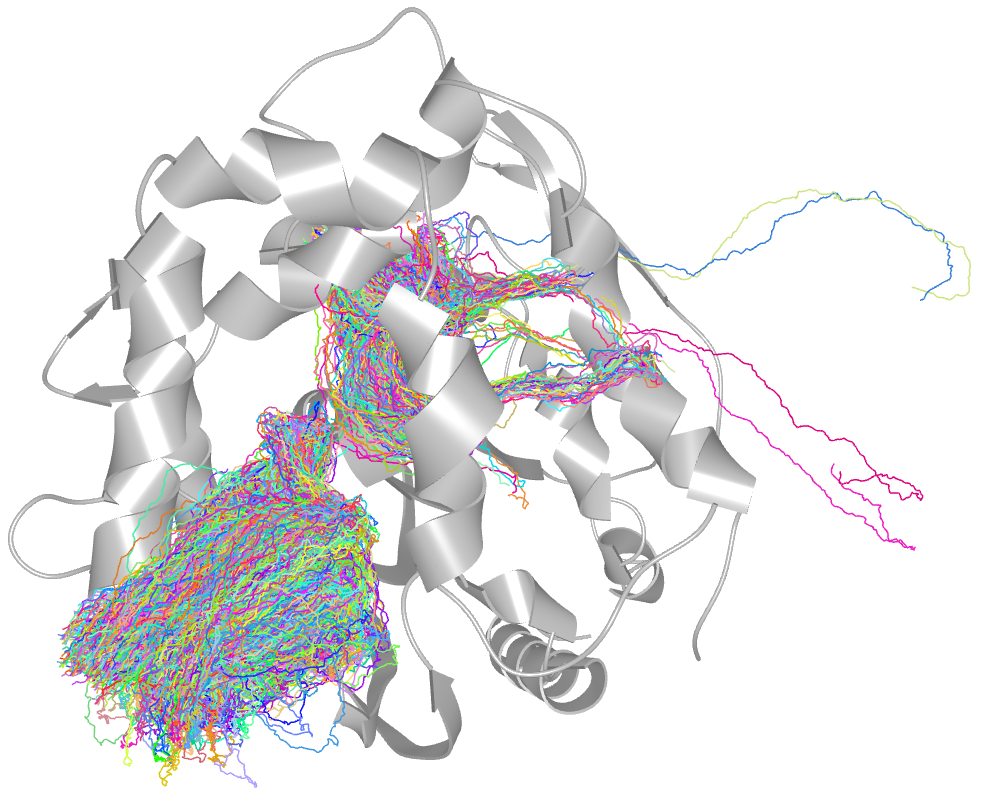
\includegraphics[width=\columnwidth]{trajectories}
  \caption{TODO replace, caption}
  \label{fig:trajectories}
\end{figure}

\subsection{Binding Energy Profile}

From the chemistry point of view, the binding energy of a ligand-substrate complex is an essential measure when evaluating the complex.
Therefore, we decided to strongly focus on conveying the binding energy when visualizing the trajectories dataset.
Naturally, this can be achieved by sampling the binding energy along a ligand trajectory and plotting the obtained data to a 2D chart.
In this manner, we obtain an abstraction of the trajectory in terms of the ligand binding energy profile (see Figure~\ref{fig:trajectory}).
Further, the energy profiles of the trajectories can be visualized within one 2D plot using superimposition.

\begin{figure}[htb]
  \centering
  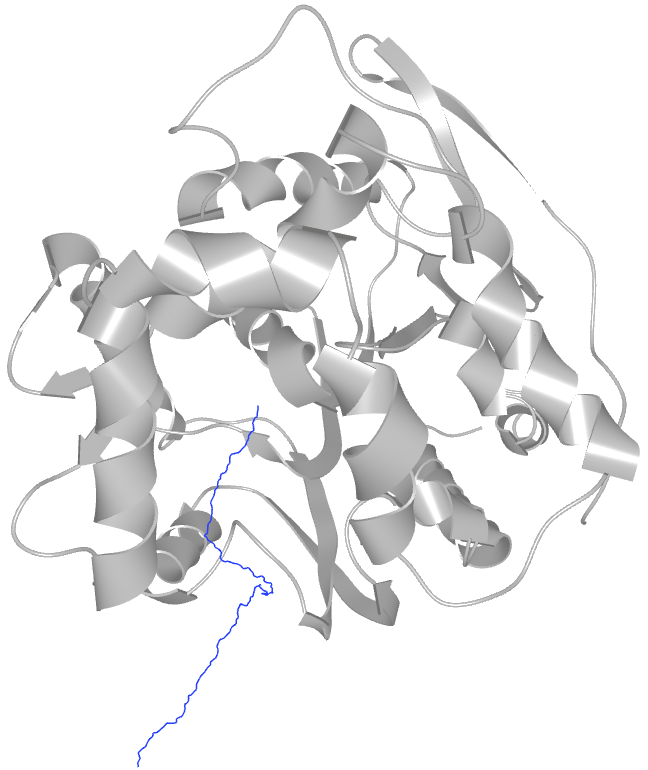
\includegraphics[width=0.5\columnwidth]{trajectory}\\
  \vspace{1em}
  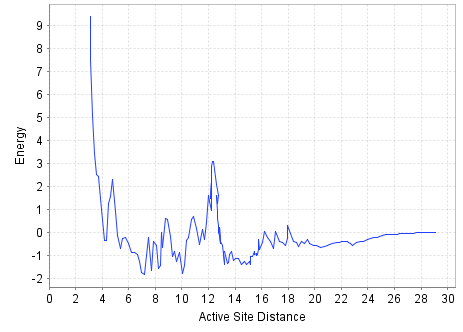
\includegraphics[width=0.8\columnwidth]{trajectory-energy}
  \caption{TODO figure quality, caption}
  \label{fig:trajectory}
\end{figure}

However, the superimposed visualization of energetic profiles does not scale well and becomes uninformative when visualizing hundreds (and more) trajectories (see Figure ?).
Particularly, there arise two issues for the users of such visualization. First, the main energetic trends become overshadowed, and second it is not possible to navigate to individual trajectories.
In order to overcome these issues, we propose a visualization system which employs well established visualization concepts in an interactive manner such that a ligand trajectories dataset can be explored based on the user needs.
Namely, we reduce the amount of energetic profiles visualized in a chart by binning the data and presenting it using small multiples~\cite{tufte1990envisioning} approach.
We bin the trajectories according to their location within a paremetric space which we define based on 1D variables that describe the trajectories (see Section~\ref{sec:multiples}).
We aim for as general as possible usage and therefore we let the user to control the variables that define the parametric space.

\section{Visual Analysis of Trajectories}

TODO
\begin{itemize}
  \item figures of direct visualization of trajectories, profiles
\end{itemize}

\subsection{Small Multiples (Dataset Slicing)}
\label{sec:multiples}

\paragraph{•} Properties -- In order to be able to slice the data, we first define an abstract representation of a ligand trajectory.
We decided to represent the trajectory using a set of 1D variables that we call trajectory properties.
Each trajectory property is defined such that it describes a specific characterstic of the trajectory.
We define the following properties:
\begin{itemize}
  \item \textbf{Minimum Distance to Active Site} --
  \item \textbf{Area Under Curve} --
  \item \textbf{?Energy Variance} --
  \item \textbf{Structure RMSD} --
  \item \textbf{Ligand Conformation Variance} --
\end{itemize}

\paragraph{•} Trends

\paragraph{•} Zooming

\subsection{3D Visualization}

\paragraph{•} Spatial Aggregation

\section{Evaluation}

TODO
\begin{itemize}
  \item LinBwt vs. LinB32 (W177 closes main tunnel)
\end{itemize}

Ve Fig 3 je videt, jak v LinBwt ligand prochazi skoro vzdycky.
Naopak ve Fig 4 je videt, ze v LinB32 ligand projde malokdy.
To odpovida laboratornim datum o snizene aktivite po mutaci (W177).

\begin{figure}[h]
  \centering
  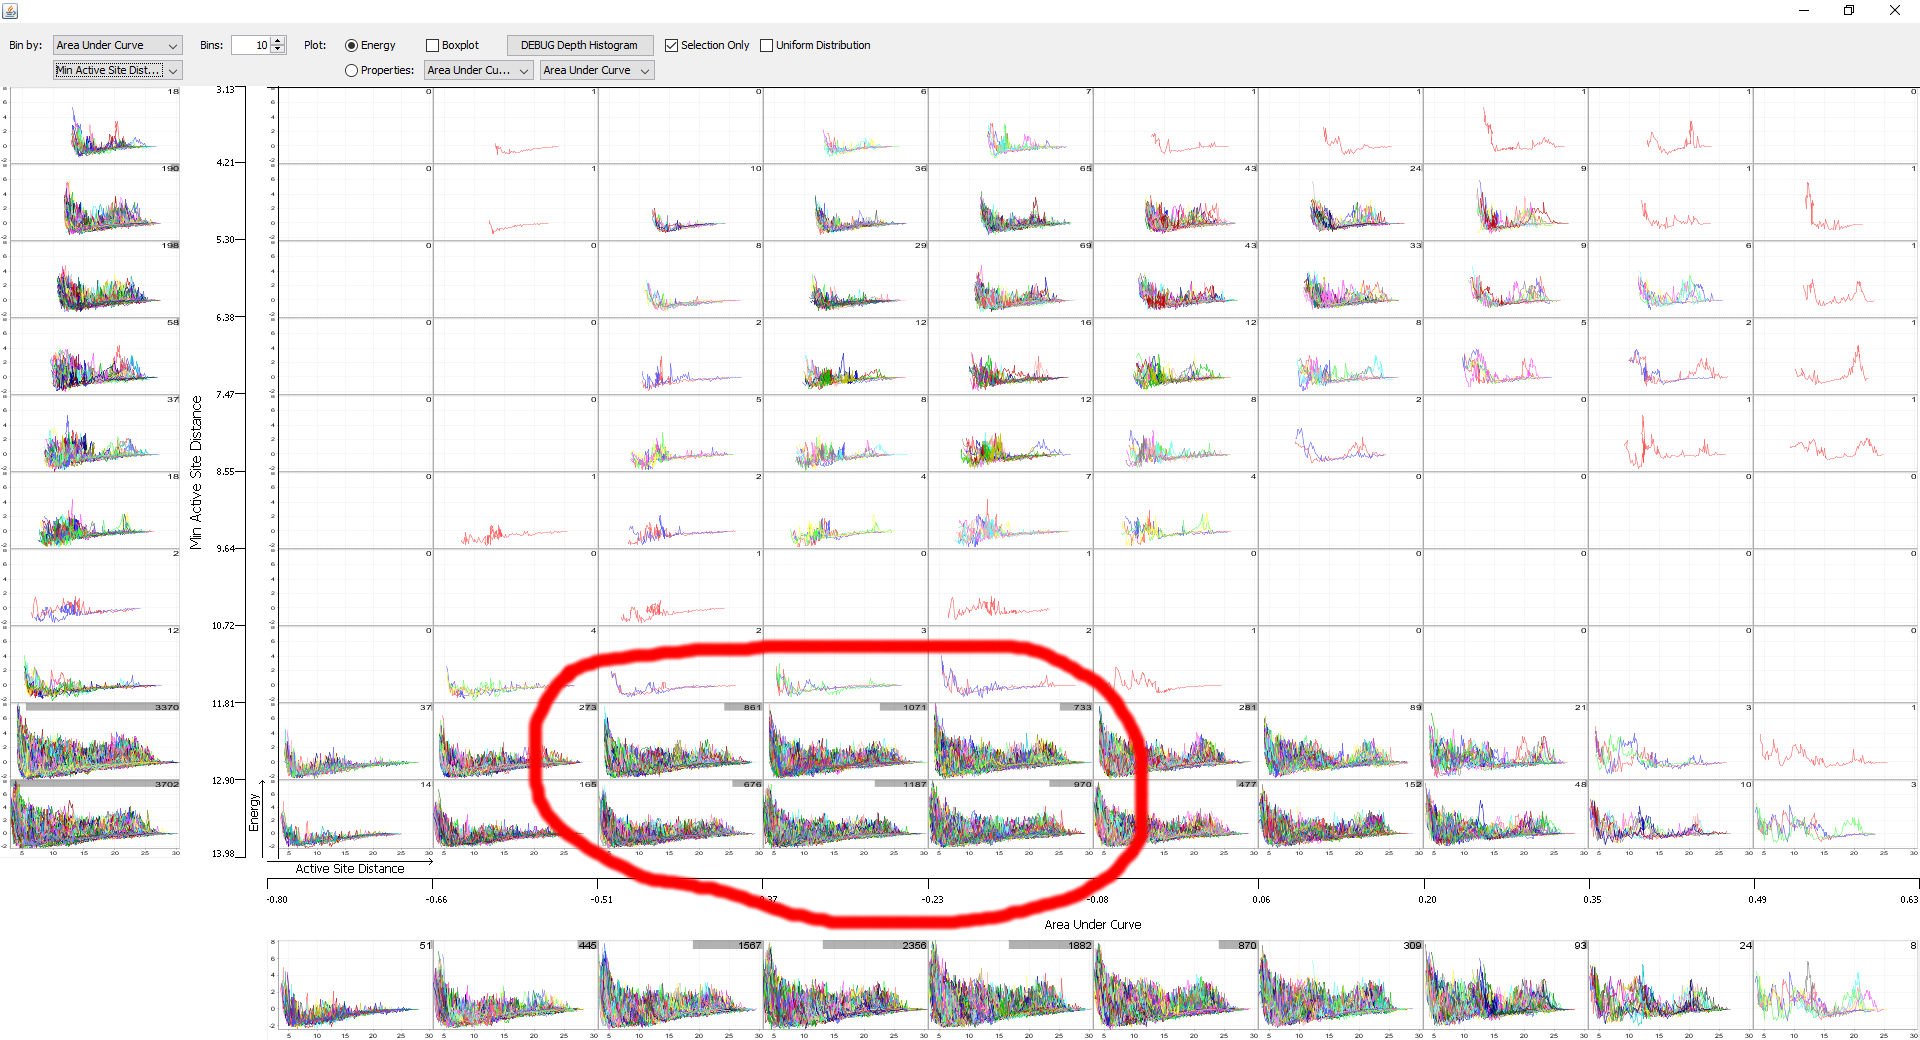
\includegraphics[width=\columnwidth]{cs01-linbwt-all}
  \caption{TODO}
\end{figure}

\begin{figure}[h]
  \centering
  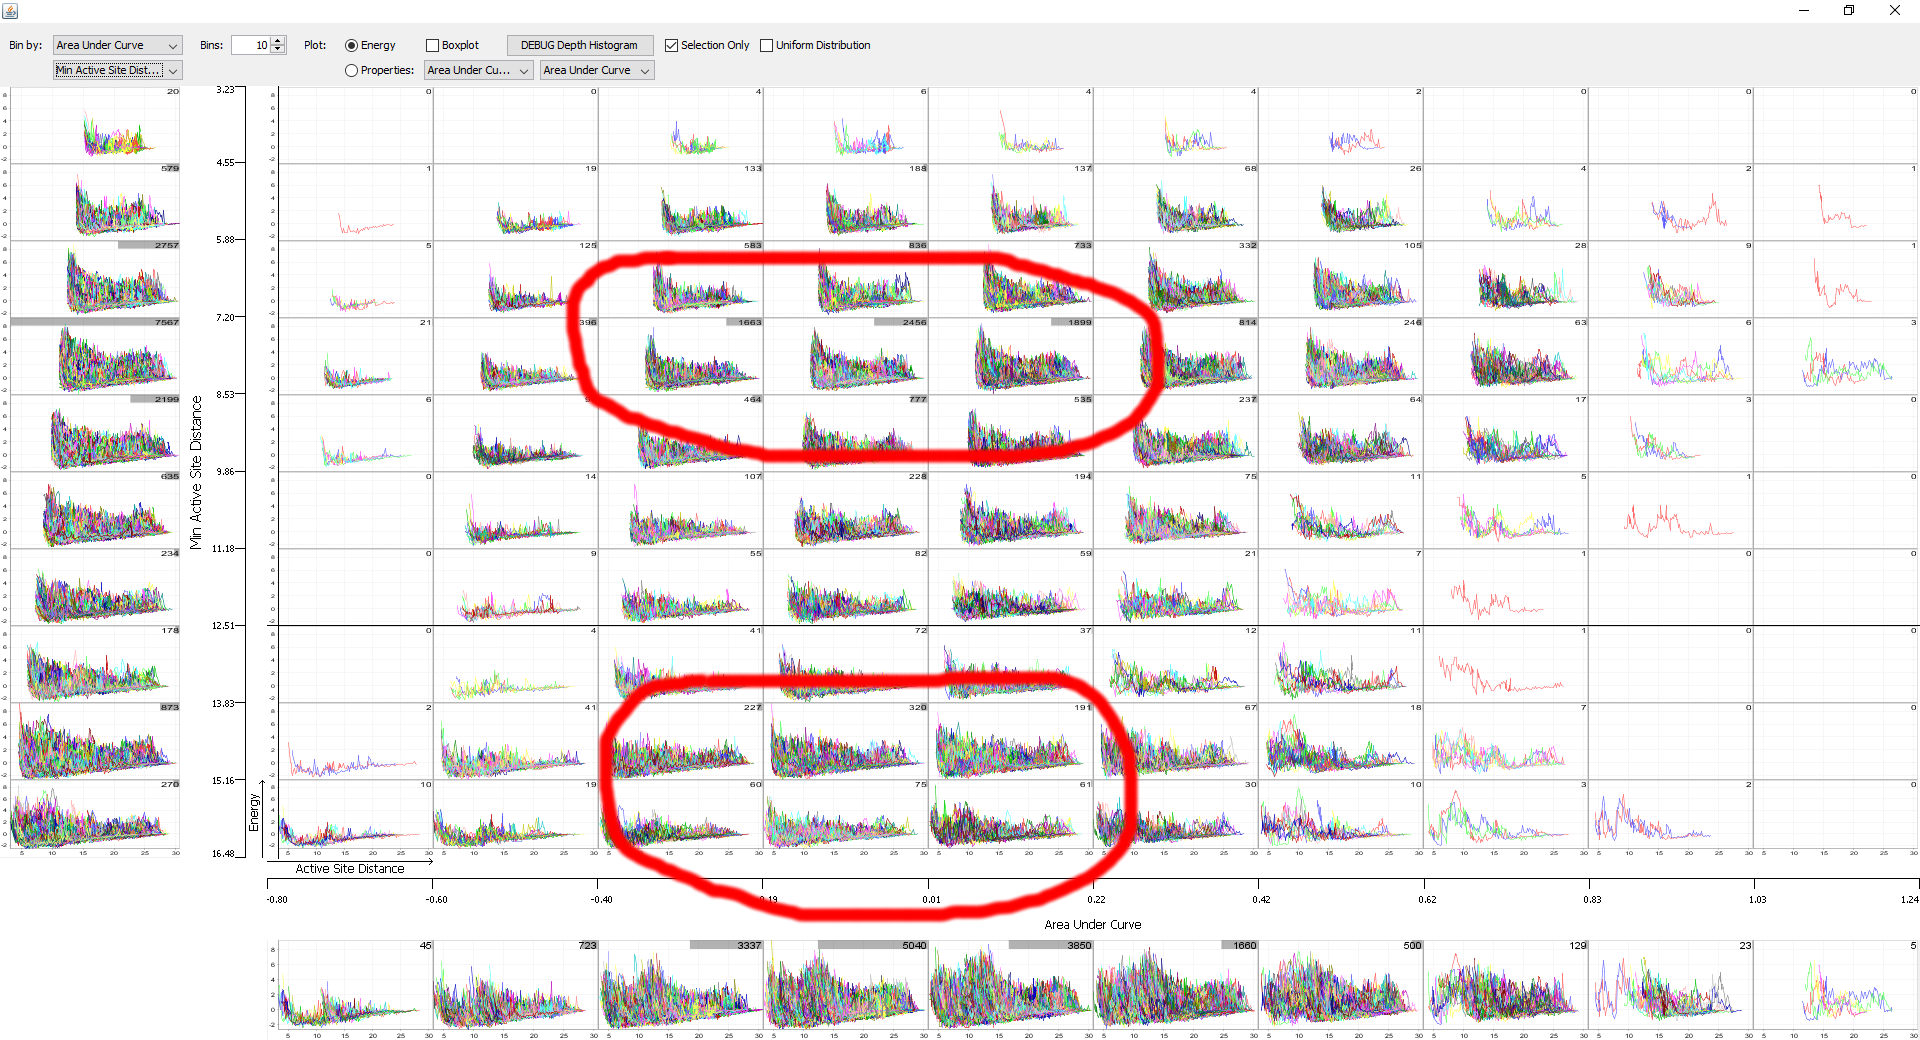
\includegraphics[width=\columnwidth]{cs01-linb32-all}
  \caption{TODO}
\end{figure}

Po prozkoumani horni skupiny u Fig 4 je videt, ze se ligandy zastavily pri pruchodu okolo mutovane W177.
Narust energie je videt na Fig 6.

\begin{figure}[h]
  \centering
  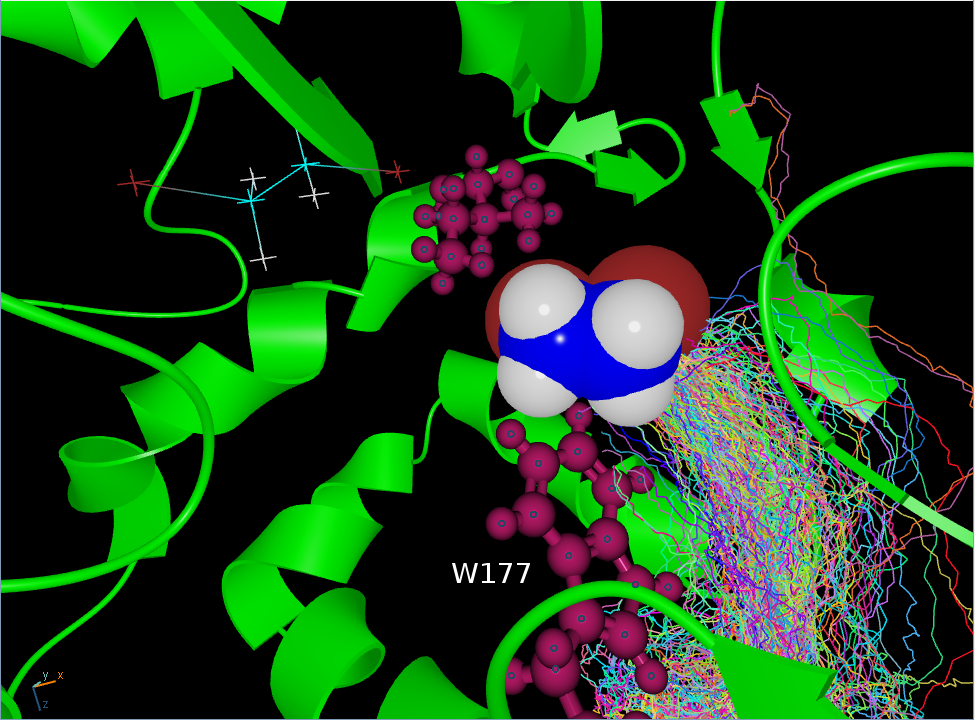
\includegraphics[width=\columnwidth]{cs01-linb32-sel-failed-3d}
  \caption{TODO}
\end{figure}

\begin{figure}[h]
  \centering
  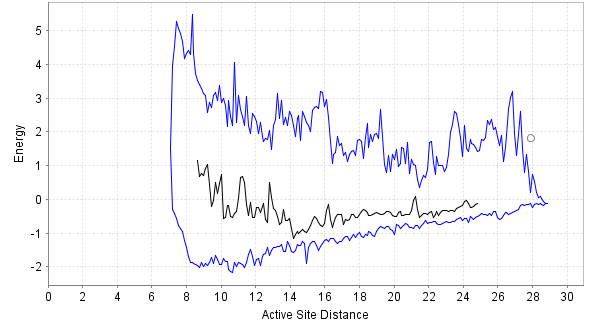
\includegraphics[width=\columnwidth]{cs01-linb32-sel-failed}
  \caption{TODO}
\end{figure}

Kdyz se podivame na trajektorie, ktere byly uspesne na LinBwt a LinB32, tak to vypada takto. Fig 7 vs. Fig 8.

\begin{figure}[h]
  \centering
  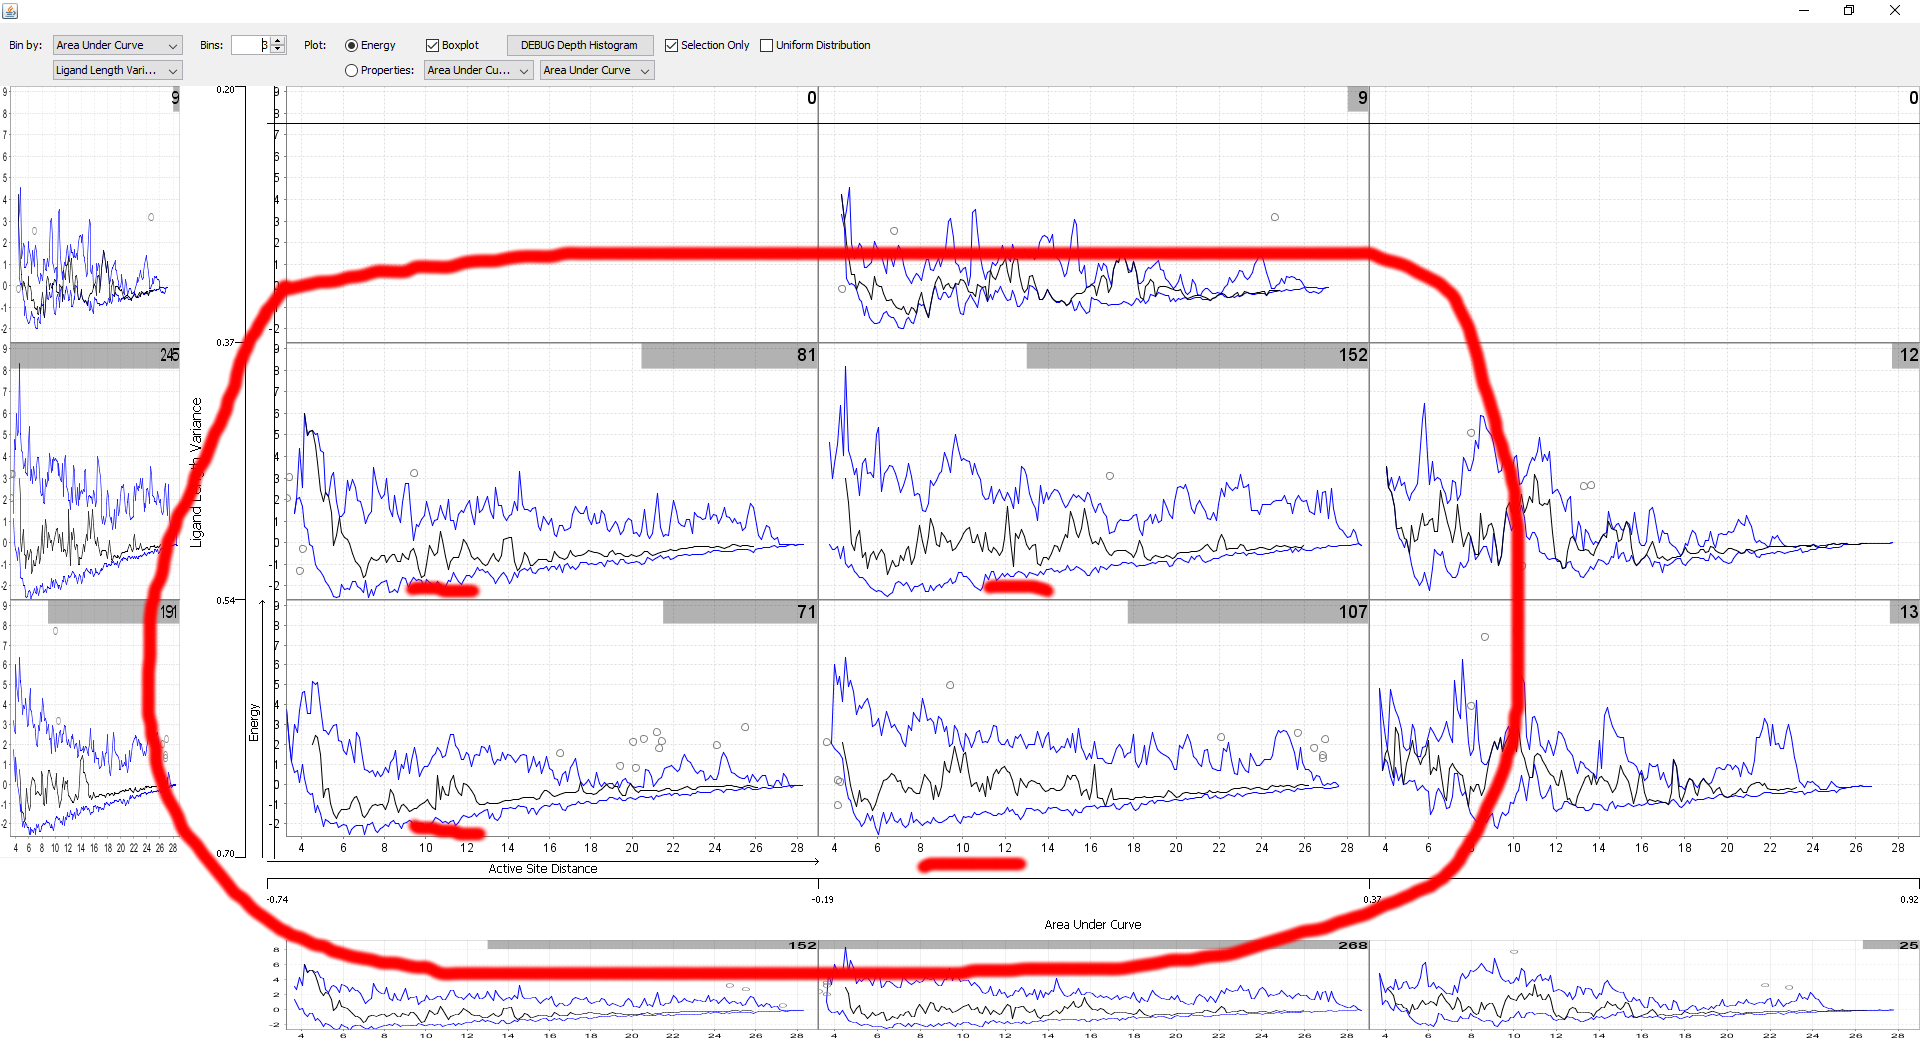
\includegraphics[width=\columnwidth]{cs01-linb32-sel-success}
  \caption{TODO}
\end{figure}

\begin{figure}[h]
  \centering
  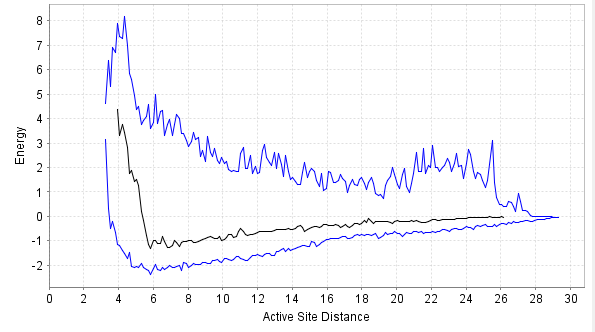
\includegraphics[width=\columnwidth]{cs01-linbwt-sel-02}
  \caption{TODO}
\end{figure}

Pri pohledu ve 3D to na LinB32 vypada takto (Fig 9).
Mutace snizila pruchodnost tunelu p1.

\begin{figure}[h]
  \centering
  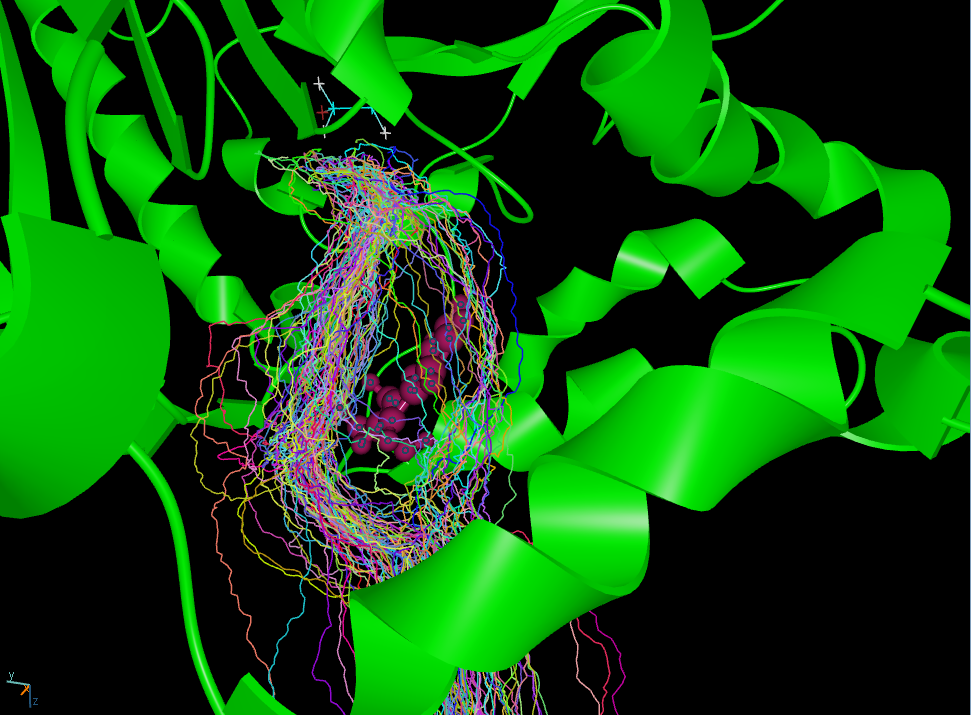
\includegraphics[width=\columnwidth]{cs01-linb32-sel-success-3d}
  \caption{TODO}
\end{figure}

Dalsi use case by mel ukazat, ze nekdy, kdyz ligand projde na LinB32, konformace molekuly se zmenila.

\section{Discussion (+ Future Work)}
\label{sec:discussion}

TODO
\begin{itemize}
  \item can be used also for CaverDock, MoMA-LigPath (Vina run needed)
\end{itemize}

\section{Conclusion}

%% if specified like this the section will be committed in review mode
\acknowledgments{TODO This work was supported in part by a grant from XYZ.}

%\bibliographystyle{abbrv}
\bibliographystyle{abbrv-doi}
%\bibliographystyle{abbrv-doi-narrow}
%\bibliographystyle{abbrv-doi-hyperref}
%\bibliographystyle{abbrv-doi-hyperref-narrow}

\bibliography{paper}
\end{document}
